\firstsection{Introduction}

\maketitle

\begin{figure*}[tb]
    \centering % avoid the use of \begin{center}...\end{center} and use \centering instead (more compact)
    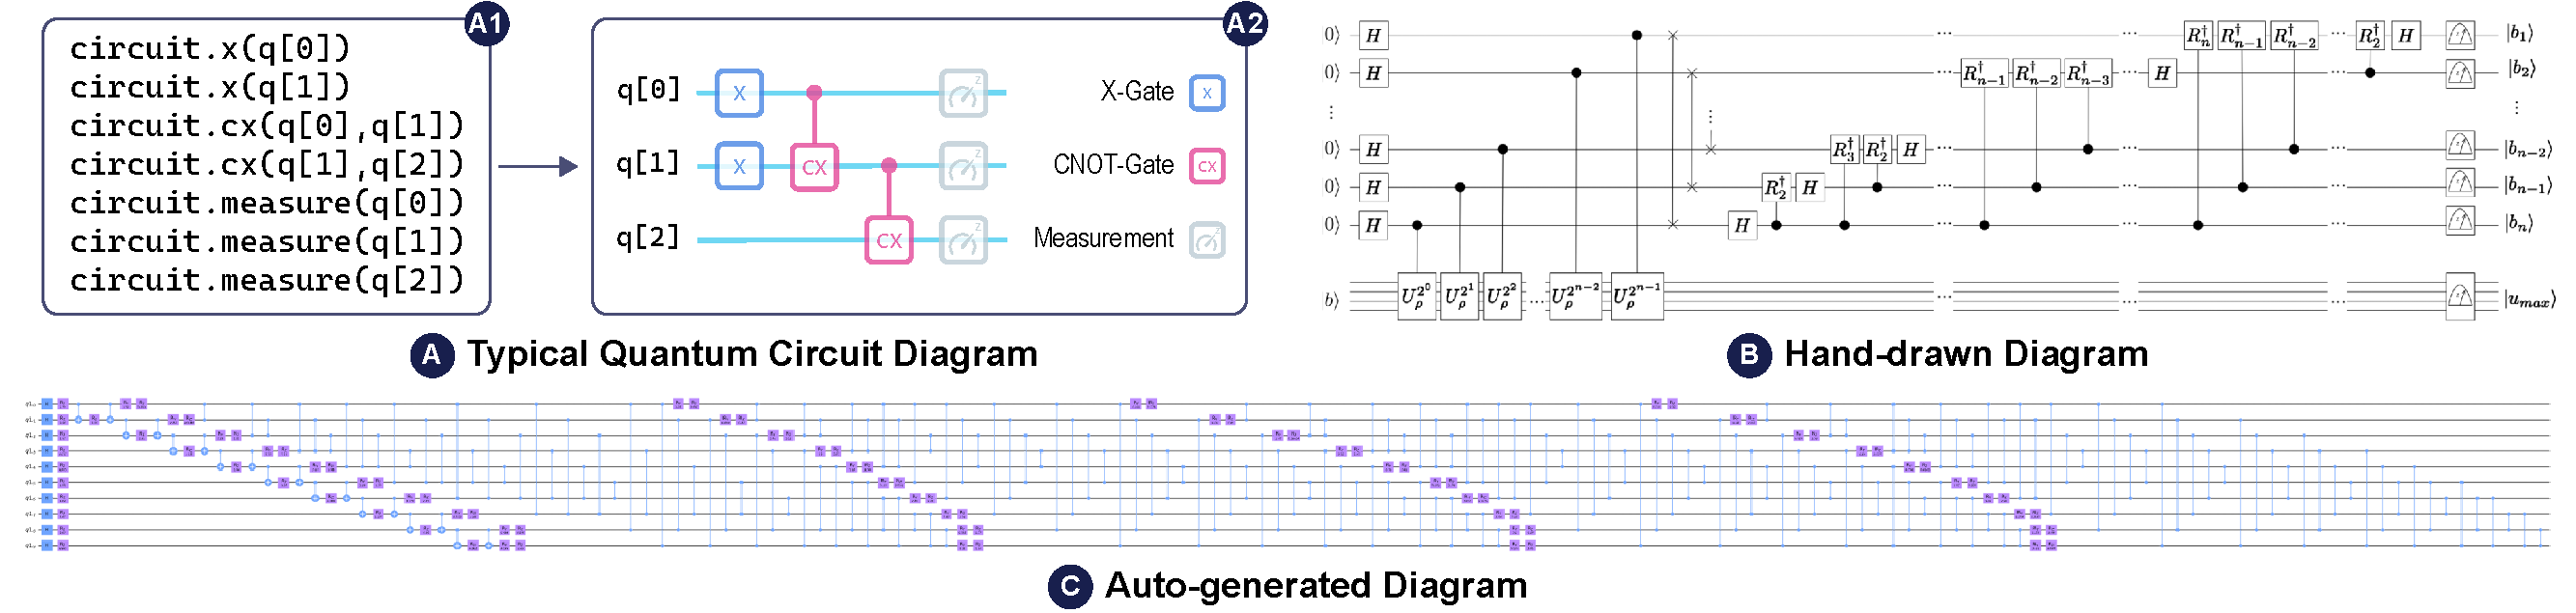
\includegraphics[width=\linewidth]{qc-samples}
    \caption{%
        The illustration of quantum circuit diagrams. (A) A typical quantum programming code (A1) and its corresponding quantum circuit diagram {(A2)}.
        (B) A hand-drawn quantum circuit diagram depicts the implementation of quantum PCA algorithm\cite{Martin:2021:TPFD}. (C) An auto-generated diagram (using Qiskit library\cite{Qiskit}) visualizes a quantum circuit having 10 qubits and 306 quantum gates.
        %
    }
    \label{fig:qc-samples}
\end{figure*}

% Quantum computers utilize the principles of quantum mechanics to perform certain computations that are more efficient than classical computers\cite{Nielsen:2010:QCBook}. Most of current available quantum computers use a computation model, called quantum circuit\cite{Deutsch:1989:QCN,Yao:1993:QCC}
% , which is employed for both the representation and implementation of quantum algorithms.
Quantum computers utilize the principles of quantum mechanics, which have the potential to outperform classical computers in certain tasks~\cite{Nielsen:2010:QCBook} when reaching hundreds of qubits.
Most current quantum computers perform calculations by executing quantum circuits, a computation model that is employed for both representation and implementation.
Emergent quantum algorithms implemented by quantum circuits suggest exponential speedup over classical algorithms, which benefits various research communities, such as finance\cite{Egger:2020:QCF}, chemistry\cite{Bauer:2020:QAQCQMS}, biological sciences\cite{Emani:2021:QBS}, and machine learning\cite{Biamonte:2017:QML, Liu:2021:QSML}.

% In the general quantum computing workflow\cite{Weder:2020:IQC}, quantum circuits are defined using quantum programming languages and libraries, such as Q\#\cite{Svore:2018:QSharp} or Qiskit\cite{Qiskit}.
% However, it is well-known that the design of quantum programs is non-intuitive ({\cref{fig:qc-samples}}-A1)\cite{Honarvar:2020:PTQP}.
In the workflow of quantum computing\cite{Weder:2020:IQC}, researchers describe quantum circuits by programming languages or libraries, such as Q\#\cite{Svore:2018:QSharp} and Qiskit\cite{Qiskit} as shown in \cref{fig:qc-samples}-A1. The compiler then transforms the code into executable quantum circuits.
As the original program can not reveal the dependencies between gates,
researchers often use quantum circuit diagrams to assist in the design of quantum algorithms.
These diagrams use time-dependent representations to visualize the structure and behavior of quantum circuits.
% {\Cref{fig:qc-samples}}-A2 shows a typical diagram that depicts a quantum program including the fundamental elements of quantum circuits, \emph{i.e.} \emph{qubits}, \emph{quantum gates}, and \emph{measurements}. 
% Each horizontal line represents a qubit which is the basic unit of information in quantum computing, analogous to a bit in classical computing. 
% The rectangular shapes on the qubits indicate quantum gates which function as operators for qubits, analogous to the role of logic gates in classical digital circuits.
% The sequence of operations follows a left-to-right order.
% Finally, the output of the quantum circuit is observed through the measurement of qubits at the end of the circuit. A well-designed quantum circuit diagram conveys an explicit explanation of a quantum algorithm.
{\cref{fig:qc-samples}}-A2 shows a typical diagram that depicts a quantum circuit including its fundamental elements, \emph{i.e.} \emph{quantum bits} and \emph{quantum gates}.
Each horizontal line in the diagram corresponds to the operation timeline of a quantum bit (or qubit).
A notation (\emph{e.g.} a square box) on the timeline specifies a quantum operation, referred to a quantum gate, that modifies the information stored in the qubits.
The execution sequence of quantum gates follows a left-to-right order.
The final information of qubits after the operations are regarded as the circuit output, which can be sent to other quantum circuits or transformed into classical information by measurement.
In summary, a quantum circuit diagram can explicitly describe a quantum computation procedure.

% However, despite the usefulness of quantum circuit diagrams, 
% Although the usefulness of quantum circuit diagrams has been proven in practice,
% creating clear and effective representations for quantum circuits still poses significant challenges.
% Currently, two techniques are commonly used to visualize quantum circuits, \emph{i.e.}, hand-drawing and automatic generation.
% Hand-drawing methods summarize quantum circuits and present semantic information through visual abstractions (\cref{fig:qc-samples}-B), whereas the manual design and creation process is time-consuming and error-prone.
% % because it requires delicate design and consistency guaranteed between the visualization and the actual quantum circuits.
% It is also tedious to update hand-drawn quantum circuits during the development process to maintain consistency between actual circuits and visualizations. 
% Some quantum computing libraries offer built-in functions for automatic circuit visualization (\cref{fig:qc-samples}-C).
% The automatic generation enables faster and more accurate circuit representation,
% and benefits for the development of small-scale quantum circuits.
The creation of quantum circuit diagrams typically involves two techniques, \emph{i.e.}, hand-drawing and automatic generation.
Hand-drawing methods summarize quantum circuits and present their semantic information through visual abstractions (\cref{fig:qc-samples}-B), whereas the manual design and creation process is time-consuming and error-prone.
Furthermore, updating the diagram when the actual circuit changes is a tedious work.
% It is also tedious to update the diagram when the actual circuit is changed. 
On the other hand, some libraries~\cite{Qiskit, Cirq} offer built-in functions for automatic visualization (\cref{fig:qc-samples}-C), which enable efficient and accurate circuit representation and benefits for the development of small-scale quantum circuits.
However, this technique is limited when scaling to a large number of qubits and quantum gates.
% but can only be scaled to a small number of qubits.
% However, direct printing of whole quantum circuits may result in extremely large outputs, and rendering details illegible.
% These techniques work well for small quantum circuits.

Recent advances in quantum computers pose significant challenges for creating clear and effective representations for quantum circuits,
as the development of quantum circuits are expanding to larger scales.
% As the advances in quantum computers, the design and implementation of quantum circuits are expanding to larger scales.
% % The current state-of-the-art quantum computers have a capability of more than 100 qubits, which enables the implementation of scalable quantum circuits.
% Although the usefulness of quantum circuit diagrams has been proven in practice, creating clear and effective representations for quantum circuits still poses significant challenges.
A number of institutions and universities have proposed quantum computers that can implement circuits with hundreds of qubits.
% , while existing visualization techniques of quantum circuits do not catch up to their pace. 
% To be specific,
% The typical quantum circuit diagrams are inadaptable for rendering large-scale quantum circuits in a limited screen space.
Nevertheless, the increasing number of qubits and quantum gates results in visual clutter and overplotting when they are visualized in typical diagrams.
For instance, {\cref{fig:qc-samples}-C} shows an auto-generated diagram that consists of only 10 qubits and 306 quantum gates, which is hard to examine.
The readability of automatically generated visualizations significantly decreases when scaling up to more than 100 qubits.
% The automatic visualization of a large-scale quantum circuit results in extremely large output, and rendering details illegible.
% The existing techniques have limitations in terms of either scalability or usability.
Therefore, an appropriate visualization approach is required to enable users to easily comprehend and analyze large-scale quantum circuits.


% Recent research in quantum computing applies classical network and graph theory to problems in complex quantum circuits\cite{Biamonte:2019:CNCQ}.
% It presents an opportunity to leverage graph visualization techniques for quantum circuit representation.
This work thus explores how visualization techniques, such as graph summarization\cite{Liu:2018:GSM} and visual abstraction\cite{Viola:2018:PCAV}, can be used for scalable quantum circuits.
Due to the complexity in deciphering quantum circuits, we introduce the semantic information to increase the readability.
To better support the goals of quantum researchers who frequently develop quantum circuits, we conduct expert interviews to understand the pain points and requirements when visualizing quantum circuits.
Inspired by findings from the interviews, we develop {\tname}\footnote[1]{\metaphor}, a {{quant}um c{i}rcuit {vi}sualizatio{n} syst{e}m} that provides efficient visual representations of large-scale quantum circuits and supports interactive exploration and analysis.
% the vast and complex landscape of quantum circuits.
% that generates comprehensible and reasonably detailed quantum circuit visualizations with easy interactions.(\Cref{fig:teaser})


{\tname} utilizes a novel pipeline that extracts latent semantics of quantum programs to automatically visualize scalable quantum circuits using graph summarization and visual abstraction techniques.
Our approach first collects meta-data and semantic information of the quantum circuit from its underlying code.
The circuit is then segmented into components based on its semantic structure, while reorganizing it through qubit bundling and gate grouping.
We also employ a semantic-preserving layout strategy in this process to ensure the new diagram is clear and easy to interpret.
Furthermore, we exploit semantic meanings of the code fragments to identify repetitive patterns in the circuit, which are subsequently presented through visual abstractions.
% These patterns are summarized from a comprehensive survey on current benchmark quantum algorithms.
These patterns are summarized from a comprehensive survey on a circuit benchmark, that covers all well-known quantum algorithms.
Lastly, we design a series of visual representations that complement contextual information to facilitate the comprehension and analysis of the quantum circuit.
% The organization and minimization of quantum circuit representation can be achieved effectively through the use of semantics.

In summary, the contributions of this research include:

\begin{itemize}
    \item We distill a list of design requirements for visualizations of large-scale quantum circuits from expert interviews.
    \item We propose a novel pipeline for visualizing quantum circuits that addresses challenges in readability and scalability with the support of semantic information and a series of visual designs.
    \item We develop {\tname}, a proof-of-concept system to demonstrate the effectiveness of our pipeline through two benchmark quantum algorithms with up to {99} qubits and an evaluation with {10} experts.
\end{itemize}

